\documentclass{article}
\usepackage[preprint]{neurips_2025}
\usepackage{graphicx,booktabs,amsmath,amssymb,caption}
\usepackage[hidelinks]{hyperref}
\captionsetup{font=small,skip=3pt}
\captionsetup[table]{position=top}
\setlength{\parskip}{3pt}
\setlength{\abovedisplayskip}{5pt}
\setlength{\belowdisplayskip}{5pt}
\title{Generating WikiArt Paintings with a DCGAN}
\author{Yu-Heng Lai \\ ECE 285, University of California San Diego}
\begin{document}
\maketitle
\begin{abstract}
We implement an unconditional deep convolutional generative adversarial network (DCGAN)
and train it on WikiArt for 50 epochs at $64\times64$ resolution.
We report loss curves, fixed-noise samples, and PyTorch-Ignite Inception Score (IS)
and FID against held-out paintings, using the course tutorial's 1,000-dimensional
class-probability protocol. The final generator reaches FID 0.0283 and IS 2.91;
held-out real paintings score 0.0125 and 3.69.
Code is available at \url{https://github.com/Lukelaitw/2026Fall-UCSD-ECE285-HW2}.
\end{abstract}

\section{Method}
The networks follow the DCGAN architecture of the PyTorch tutorial~[3].
A generator maps $z\sim\mathcal{N}(0,I_{100})$ to an RGB image:
five kernel-4 transposed convolutions expand the spatial size from $1$ to
$4,8,16,32,64$ with hidden channels $512\!\to\!256\!\to\!128\!\to\!64$, using batch normalization and ReLU
in hidden layers and tanh at the output.
The discriminator mirrors it with stride-2 convolutions, batch normalization except at
the input and output, and LeakyReLU$(0.2)$; its final convolution returns one logit per image.
The generator and discriminator have 3,576,704 and 2,765,568 parameters.
Each minibatch takes one discriminator step, then one non-saturating generator step:
\[
L_D=-\mathbb{E}_{x}\log\sigma(D(x))-\mathbb{E}_{z}\log\bigl(1-\sigma(D(G(z)))\bigr),\qquad
L_G=-\mathbb{E}_{z}\log\sigma(D(G(z))),
\]
computed as binary cross-entropy on logits; fake images are detached for the discriminator step.
Convolution weights are initialized from $\mathcal{N}(0,0.02^2)$ and
batch-normalization scales from $\mathcal{N}(1,0.02^2)$, with zero biases.

\section{Data and training setup}
The images come from the assigned Kaggle WikiArt collection~[1]. All discovered images were selected.
A seed-42 image-level split uses 65,155 images for training and 16,289 held out.
Images are oriented using EXIF, converted to RGB, bilinearly resized so the
shorter edge is 64, center cropped to $64\times64$, and scaled to $[-1,1]$.
Labels are unused and no augmentation is applied.

\begin{center}
\small
\captionof{table}{Training configuration. The last, smaller minibatch of each epoch is kept.}
\begin{tabular}{llll}
\toprule
Latent size / base channels & 100 / 64 & Batch size / epochs & 128 / 50 \\
Optimizer / learning rate & Adam / 0.0002 & Adam $(\beta_1,\beta_2)$ & $(0.5,0.999)$ \\
Seed / training device & 42 / cuda & Updates per network & 25,500 \\
\bottomrule
\end{tabular}
\end{center}

\section{Training behavior}
Figure~\ref{fig:loss} shows per-epoch means weighted by minibatch size.
In the final epoch, $L_G=3.5863$, $L_D=0.4469$, $D(\text{real})=0.8511$,
and $D(\text{fake})=0.1488$, with probabilities taken before each discriminator update.
% Observation for outputs/dcgan_wikiart_e050; recheck it before reusing this template.
$L_G$ falls steeply in the first few epochs and more slowly until about epoch 30.
Afterwards it drifts upward, apart from a brief dip at epoch 42, while
$D(\text{real})$ rises and $D(\text{fake})$ falls: the discriminator slowly gains.
The two objectives need not decrease together, so loss alone does not measure quality;
the final checkpoint still has the lowest FID in Table~\ref{tab:scores}.

\begin{figure}[t]
\centering
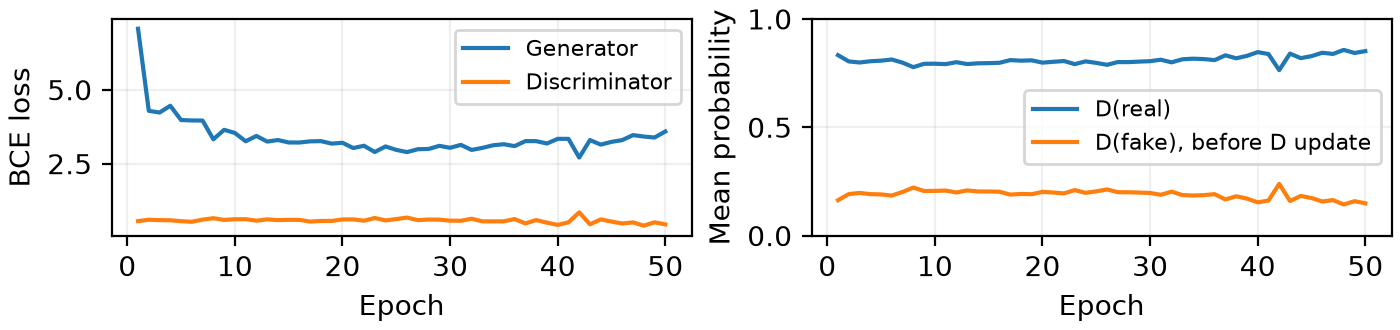
\includegraphics[width=\linewidth]{figures/loss.png}
\caption{Generator/discriminator losses and mean discriminator probabilities per epoch.}
\label{fig:loss}
\end{figure}

\section{Evaluation and generated examples}
We score the checkpoints in Table~\ref{tab:scores}, ending with the final epoch-50
checkpoint, with PyTorch-Ignite 0.5.5 as in the course tutorial~[2].
A real reference set and a disjoint real control set each hold 2,000 randomly chosen
held-out images, unused in training; every checkpoint generates from the same 2,000
standard-normal latent vectors, independent of the fixed sample grid.
FID compares a set with the reference and IS uses the set alone, so the real control
shows what real paintings score.
Images are mapped from $[-1,1]$ to $[0,1]$, quantized to uint8, bilinearly resized with
PIL to $299\times299$, and given to Inception-v3 as floats in $[0,1]$ without mean/std
normalization, as in the tutorial. The features are ImageNet class probabilities
(1,000 dimensions), not the usual 2,048-dimensional pool3 features, and IS is the
aggregate Ignite score without split averaging.

\begin{center}
\small
\captionof{table}{IS and FID against the held-out reference (2,000 images per set); comparable only within this protocol.}
\label{tab:scores}
\begin{tabular}{lccccc@{\qquad}c}
\toprule
Generator after epoch & 10 & 20 & 30 & 40 & 50 & Real control \\
\midrule
FID $\downarrow$ & 0.0960 & 0.0370 & 0.0374 & 0.0361 & 0.0283 & 0.0125 \\
IS $\uparrow$ & 2.36 & 2.66 & 2.90 & 2.92 & 2.91 & 3.69 \\
\bottomrule
\end{tabular}
\end{center}

% Observation for outputs/dcgan_wikiart_e050; recheck it before reusing this template.
The fixed-noise samples in Figure~\ref{fig:samples} include portrait-like, landscape,
seascape, sketch, and abstract compositions with no visible mode collapse,
but faces and figures are distorted at this resolution.

\begin{figure}[t]
\centering
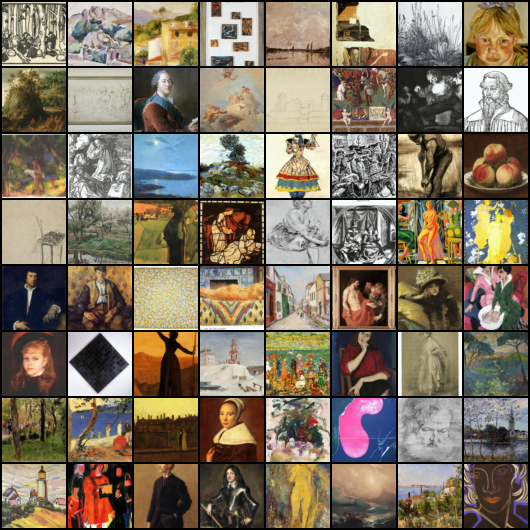
\includegraphics[height=1.8in]{figures/real.png}\hspace{0.25in}%
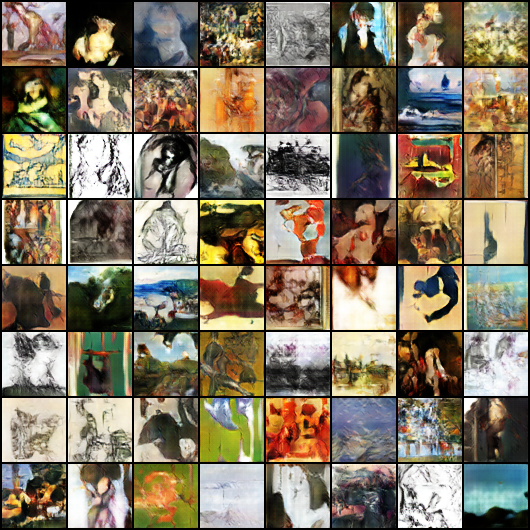
\includegraphics[height=1.8in]{figures/generated.png}
\caption{Left: the first 64 images of the seeded training split.
Right: 64 unfiltered outputs from the final generator, using the same fixed
noise vectors as every saved epoch. Quantitative scores use independent draws.}
\label{fig:samples}
\end{figure}

\section{Limitations}
The image-level split does not separate artists or remove near duplicates, and the
real control measures sampling variation rather than a universal quality floor.
ImageNet class probabilities describe paintings only coarsely, so IS and this FID cannot
establish artistic quality, originality, or coverage of every style, nor be compared
with published pool3 FID. Center cropping discards image borders,
$64\times64$ output cannot resolve fine brushwork, and all results come from one training seed.

\vspace{3pt}
{\footnotesize\raggedright
\noindent [1] WikiArt dataset. \url{https://www.kaggle.com/datasets/steubk/wikiart}.\newline
[2] PyTorch-Ignite. GAN evaluation using FID and IS.
\url{https://pytorch-ignite.ai/blog/gan-evaluation-with-fid-and-is/}.\newline
[3] PyTorch. DCGAN tutorial.
\url{https://docs.pytorch.org/tutorials/beginner/dcgan_faces_tutorial.html}.\par
}
\end{document}
